Implementamos dos algoritmos que nos ofrecen siempre que la haya una solución válida, más o menos cercana al óptimo.
En concreto un algoritmo de tipo Greedy y otro de Búsqueda Local, caracterizándose respectivamente por ir cogiendo de entre
los puntos no escogidos los que menos dispersión resultan y por partir de una solución inicial aleatoria e ir buscando de
entre los vecinos el primer mejor que mejora la dispersión de la solución que se mantenga en ese momento hasta haber llegado
a un número determinado de iteraciones o hasta no encontrar vecinos que mejoren la dispersión de la solución.

\section{Aproximación Greedy}

Como hemos mencionado anteriormente la estrategia detrás de nuestra aproximación Greedy es la de ir seleccionando
el punto que minimizaría la dispersión de la solución de entre los no seleccionados parando de añadir puntos a la
solución cuando esta fuese una solución válida. Podemos definir el algoritmo en pseudo-código como sigue:

\begin{minipage}{\textwidth}
\begin{lstlisting}[mathescape=true,caption={Definición del algoritmo Greedy.},captionpos=b]
def selecciona_punto_siguiente(solucion, puntos_no_escogidos):
    elemento_siguiente = puntos_no_escogidos[0]
    dispersion_del_elemento_siguiente = $ + \infty  $
    
    por cada punto p en puntos_no_escogidos:
        dispersion = solucion.calcula_dispersión_de_punto_candidato(p)
        si dispersion < dispersion_del_elemento_siguiente:
            elemento_siguiente = p
            devuelve elemento_siguiente
    
    devuelve elemento_siguiente

def solve(numero_de_puntos_a_elegir, mapa_distancias):
    solucion = new Solucion.asocia(mapa_distancias)
    puntos_no_escogidos = new Set.init(Rango(0, mapa_distancias.numero_de_puntos()))

    primer_punto = escoger_aleatorio(puntos_no_escogidos)
    solucion.inserta_punto_en_solucion(primer_punto)
    puntos_no_escogidos.elimina(primer_punto)
    por cada punto a elegir - 1:
        punto_escogido = selecciona_punto_siguiente(solucion, puntos_no_escogidos)
        solucion.inserta_punto_en_solucion(punto_escogido)
        puntos_no_escogidos.elimina(punto_escogido)
    
    devuelve solucion
\end{lstlisting}
\end{minipage}

Recordemos que la inserción y eliminación de un punto se realiza en tiempo $ \Theta (m) $ en una solución
y en tiempo $ O (\log n) $ en un conjunto. El cálculo de la dispersión de un nodo candidato también se realiza
en tiempo $ \Theta (m) $.

\section{Aproximación por Búsqueda Local del Primer Mejor}

El objetivo de los algoritmos de Búsqueda Local es el de examinar exhaustivamente el espacio de soluciones próximo
a una solución determinada. El criterio de parada suele involucrar un máximo de iteraciones o la imposibilidad de encontrar
soluciones entre los vecinos. Es muy bueno por tanto encontrando óptimos, pero generalmente locales debido a la naturaleza del proceso
de generación de soluciones alternativas, ya que únicamente busca entre los vecinos contiguos. Por sí solos este tipo de
algoritmos veremos que no ofrecen soluciones mucho mejores a soluciones de tipo Greedy, y que al igual que estos la
calidad de la solución vendrá muy determinada por el conjunto inicial, que se escoge aleatoriamente.

\begin{minipage}{\textwidth}
\begin{lstlisting}[mathescape=true,caption={Definición del algoritmo de Búsqueda Local.},captionpos=b]
def primer_mejor_vecino_quitando_punto_de_solucion(punto_a_quitar, solucion, puntos_no_escogidos):
    solucion_sin_punto = solucion
    solucion_sin_punto.elimina_punto_de_solucion(punto_a_quitar)

    mejor_punto = punto_a_quitar
    mejor_dispersion = solucion.calcula_dispersion()

    por cada punto p en puntos_no_escogidos:
        dispersion = solucion_sin_punto.calcula_dispersion_de_punto_candidato(p)
        si dispersion < mejor_dispersion:
            mejor_punto = p
            devuelve mejor_punto
    
    devuelve punto_a_quitar

def solve(numero_de_puntos_a_elegir, mapa_distancias):
    solucion = new Solucion.asocia(mapa_distancias)
    puntos_no_escogidos = new Set.init(Rango(0, mapa_distancias.numero_de_puntos()))
    inicializa_solucion_aleatoriamente(solucion, puntos_no_escogidos, numero_de_puntos_a_elegir)

    dispersion = $ + \infty $
    mejor_dispersion = solucion.calcular_dispersion()

    mientras mejor_dispersion < dispersion y num_iteraciones < 100.000:
        dispersion = mejor_dispersion
        por cada punto p en solucion:
            supuesto_mejor_punto = primer_mejor_vecino_quitando_punto_de_solucion(p, solucion, puntos_no_escogidos)
            si supuesto_mejor_punto es distinto de p:
                puntos_no_escogidos.inserta(p)
                puntos_no_escogidos.elimina(supuesto_mejor_punto)
                solucion.elimina_punto_de_solucion(p)
                solucion.inserta_punto_en_solucion(supuesto_mejor_punto)
                mejor_dispersion = solucion.calcula_dispersion()
\end{lstlisting}
\end{minipage}

En el capítulo segundo podemos ver que los métodos que nos proporciona la estructura de datos que hemos declarado y definido para representar y hacer
operaciones hacen que la solución esté factorizada según se indica en los requisitos de la práctica. 

\subsubsection{Métodos de exploración del entorno y operador de generación de vecino}

Como hemos mencionado anteriormente nuestro algoritmo parte de una primera solución aleatoria y a partir de esta empieza
a comparar esta solución con soluciones que va generando pertenecientes al espacio de búsqueda y cercanas a esta. Sustituye
a la solución elegida con el primer mejor vecino que encuentre.

Podemos ver en la función \texttt{primer\_mejor\_vecino\_quitando\_punto\_de\_solucion} del listado 3.2 el algoritmo
para generar soluciones adyacentes dada una solución, de forma que devuelve la primera mejor solución que encuentre.

Intuitivamente se podría describir como si cogiésemos una solución y le quitásemos un punto que pertenezca a esta.
Una vez hecho esto calculamos la dispersión que tendría una posible solución con cada uno de los puntos pertenecientes
al conjunto de los no escogidos. Si encontramos un punto no seleccionado con mejor dispersión devolvemos la solución
con ese punto, en caso contrario devolvemos la solución original. Cabe destacar que esta descripción es aproximada,
no es lo que se describe exactamente en el algoritmo.

\begin{figure}[ht]
    \centering
    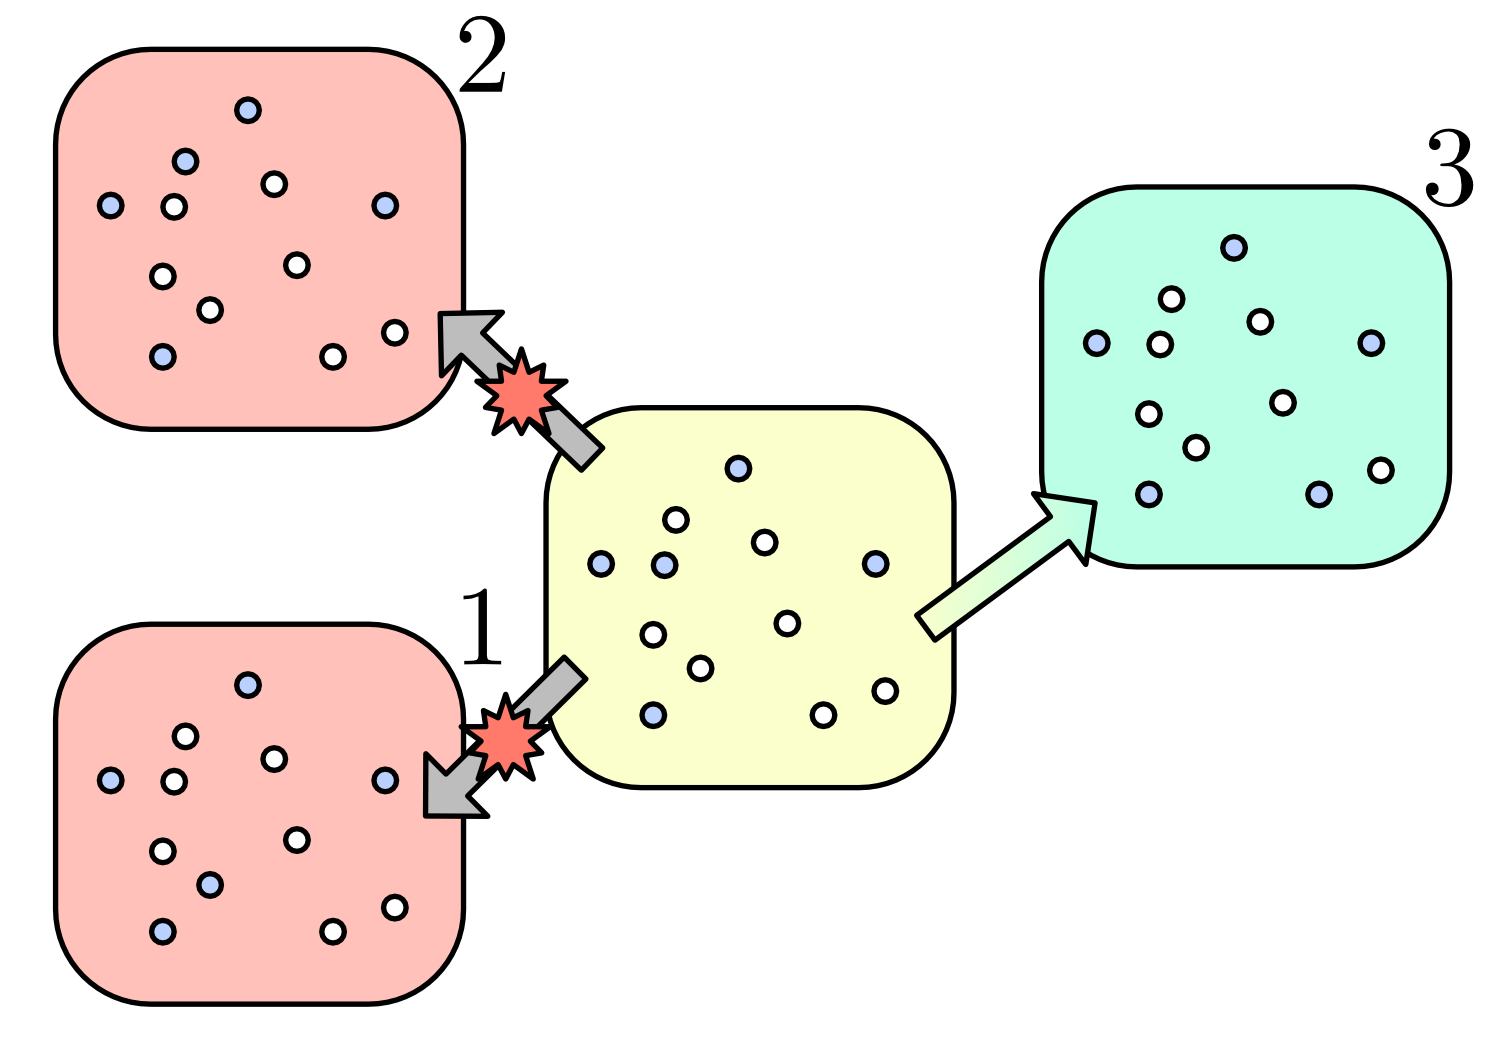
\includegraphics[height=7.5cm,keepaspectratio]{busqueda_local_exploracion.png}
    \caption{Generación y selección de vecinos en el algoritmo de Búsqueda Local Primero el Mejor. Las soluciones se generan en el orden 1, 2, 3. En el momento en el que encuentra una solución, la tercera en este caso, la devuelve.}
\end{figure}

\subsubsection{Generación de soluciones aleatorias}

En el listado 3.2 hacemos referencia a una función llamada \texttt{inicializa\_solucion\_aleatoriamente}.
La definimos en el siguiente listado.

\begin{minipage}{\textwidth}
\begin{lstlisting}[mathescape=true,caption={Definición de la función \texttt{inicializa\_solucion\_aleatoriamente} para generar una solución consistente en elementos aleatorios.},captionpos=b]
def inicializa_solucion_aleatoriamente(solucion, puntos_no_escogidos, numero_de_puntos_a_elegir):
    por cada uno de los puntos que tenemos que elegir:
        punto_elegido = escoge_aleatorio(puntos_no_escogidos)
        puntos_no_escogidos.elimina(punto_elegido)
        solucion.inserta_punto_en_solucion(punto_elegido)
\end{lstlisting}
\end{minipage}